
\documentclass{article}

\title{An Exact Method of Solving PDEs}
\author{Brent Baccala\footnote{Email address: \tt cosine@freesoft.org}}

\usepackage{amsmath}
\usepackage{amsfonts}

\usepackage{xcolor}
\usepackage{comment}

\usepackage[hidelinks]{hyperref}

\usepackage{tabularx}

\usepackage{longtable}

% For drawing ansatz diagrams

\usepackage{tikz}
\usetikzlibrary{calc}
\usetikzlibrary{positioning}
\usetikzlibrary{fit}
\usetikzlibrary{backgrounds}
\usetikzlibrary{shapes.multipart}

\def\coeff{\framebox(10,10){}}
\newcommand{\tikzmark}[1]{\tikz[overlay,remember picture] \node (#1) {};}
\def\R32003{$F_{32003}$}

\begin{document}
\parindent 0pt

\maketitle

\begin{abstract}
The author has developed an algorithm, based on differential algebra,
for finding exact, non-separable solutions of partial differential equations.
\end{abstract}

\parskip 12pt

% \subsection*{Introduction}

% An January 2023, I discovered a previously unknown solution to the simplest Schrödinger equation for the hydrogen atom.
%
% It turns out that this wavefunction:
%
% \begin{equation}
% \Psi = J_0(2\sqrt{x+r})
% \end{equation}
%
% where $J_0$ is the ordinary Bessel function $J_0$, solves the Schrödinger equation for hydrogen:
%
% \begin{equation}
% -\frac{1}{2}\nabla^2 \Psi - \frac{1}{r}\Psi = E \Psi
% \end{equation}
%
% with E=0.
%
% This paper explains the solution technique, which is generally applicable to all PDEs.
%
% %\begin{comment}
% A short list of methods to find exact solutions to PDEs:
%
% \begin{itemize}
% \item separation of variables
%
% Assume that the solution is a product of simpler functions, each of which depends on a subset of the variables
% \item method of characteristics
% \item transform methods (Fourier transform on space variables)
% \item symmetry methods
% \item calculus of variations
% \item Evans: Laplace's eq is invariant under rotations, so look for functions of r; this is a variant of sep of var
% \item Evans: Poisson's eq: Green's function is constructed from radially symmetric solution to Laplace's eq
% \item Evans: Poisson's eq: calculus of variations; show that solution minimizes a functional
% \item Evans: heat eq: uses several scaling symmetries to justify solution form depending on a single expression
% \item Evans: Duhamel's principle: separate out one variable (t) that appears like $u_t - Lu = f$ (L has no time deriv);
%       form the ``retarded solution'' that represents the effect of an infinitesimal $f$, then integrate over time
% \item Evans: heat eq: scaling symmetry $\rightarrow$ fundamental sol $\rightarrow$ convolution to handle arbitrary initial condition
%       $\rightarrow$ Duhamel's principle to handle the inhomogenous component
% \end{itemize}
% %\end{comment}
%
% \begin{comment}
% A short list of methods to find exact solutions to PDEs includes separation of variables,
% the method of characteristics, transform methods (including Fourier transforms),
% symmetry methods, Green's functions, Duhamel's principle, and the calculus of variations.
% The author has developed another exact solution technique based on differential algebra
% and has used it to find a new solution to one of the most well-studied equations
% in mathematical physics, the Schr\"odinger equation for hydrogen.
% \end{comment}

\subsection*{Introduction}
%% \subsection*{Differential Algebra}

We can construct polynomial rings (commutative, with unity) and fields using indeterminates, such as $\mathcal{Q}[x,y,z]$,
treating the indeterminates $x$, $y$, and $z$ mearly as elements of the ring that satisfy
its basic ring axioms.  We call this ``commutative algebra''.

We can then consider mapping the indeterminants into the coefficient field, and ask questions like,
Which values of $x$ in $\mathcal{Q}$ satisfy $x^2=4$?  We can consider systems of polynomial
equations, and seek to describe which values of indeterminates satisfy all of the equations
in the system.  We introduce ideals in the polynomial ring and algebraic varieties in the
solution space and deduce the contravariant equivalence between them.  We call this
``algebraic geometry''.

J.F. Ritt introduced differential algebra \cite{Ritt}.
Given a ring $R$ (commutative, with unity) or a field $F$, we can construct a
{\it differential ring} or {\it differential field}
by specifying one or more derivations that commute
with addition and obey the Leibniz rule for multiplication [Ritt]:

\begin{equation*}
D(ab) = (Da)b + a(Db)
\end{equation*}

Various notations are in common use for the derivations;
%, including
%the letter $D$, apostrophes and/or superscripted numbers if only
%a single derivation is in use (the ODE case), or
I generally use``jet notation'' where derivations are denoted by subscripted letters, i.e, $\Psi_x$
is the result of applying derivation $x$ (a unary operator)
to $\Psi$.  Analytically, we will always interpret this as the derivative
of $\Psi$ with respect to $x$;
thinking of the derivation as a unary operator
is an algebraic concept.  The distinction is much the same
as between the real number $\sqrt{2}$ and the element $\gamma$
in the algebraic extension of $\mathbb{Q}$ defined by the polynomial equation $\gamma^2=2$.

% The Risch algorithm

% The use of differential Galois theory to analyze linear ODEs.

% The failure of differential Galois theory to answer the obvious question about PDE.

Combining the concepts of differential algebra and algebraic geometry together,
we obtain {\it differential algebraic geometry},
where we have systems of differential polynomials and seek find solutions when the
indeterminates are mapped to... what?

Mapping the indeterminates to constants, for example the complex numbers, isn't a fruitful
course of action since the derivatives of constants are always zero, so likewise will
our derivations map constants to zero.  Instead, we map the indeterminates to functions
in some function space.  Exactly which function space we use
depends on the specific problem.
Popular choices include complex analytic on $C^n$, or $H^2(R^n)$.
%Much as in the case of algebraic geometry, it is often most convenient
%to map indeterminates into the coefficient field, we can let the coefficient field
%be the function space.  This is by far the most common approach in differential algebraic geometry.

However, I find it useful to consider the function space as something quite
small, parametized by a finite number of constants, that we pick for our purpose of solving some particular
equation or system of equations.  The great advantage of this approach is that by using
a finite number of parameters to describe our function space, we can
use the tools of algebraic geometry to characterize the
solutions as algebraic varieties.

We do this by introducing
additional differential polynomials into our system.
This doesn't let use easily restrict to
something like $L^2$, because that requires imposing a global integral condition,
and there's no way to specify that using only differential polynomials.
We can, however, restrict the function space by requiring the solutions
to satisfy additional differential equations.

An algorithm begins to suggest itself.  To solve a given differential equation,
we pick a small function space
parameterized by a finite number of constants, describe it using a
system of differential polynomial equations, then use
some kind of a reduction algorithm on the original equation to extract a system of polynomial equations involving
only the constants.

What kinds of small function spaces are useful?
Starting with a PDE, I have obtained good results by restricting it to be solved using
ODEs of certain limited forms.  Parametizing those forms with a finite number
of constants yields a function space parametized by constants, and therefore
describing a solution variety in something like $\mathbb{C}^n$.  Such a
solution space is then ammenable to the techniques of algebraic geometry,
such as primary decomposition.
Each associated prime ideal in the resulting primary decomposition can be interpreted as a family
of solutions of the differential equation in the function space.

Starting, for example, with the following Schr\"odinger equation for hydrogen:

\begin{equation}
% \label{schrodinger hydrogen}
-\frac{1}{2}\nabla^2 \Psi - \frac{1}{r}\Psi = E \Psi
\end{equation}

We can require the solution to solve the following parametized ODE:

\begin{equation}
\begin{gathered}
(a_0 + a_1 v) \Psi_{vv} + (b_0 + b_1 v) \Psi_v + (c_0 + c_1 v) \Psi = 0
\end{gathered}
\end{equation}

where $\Psi(v)$ is a univariate function of some variable $v$, itself expressed in a parameterized form:

\begin{equation}
% \label{ansatz 5a}
v = v_1 x + v_2 y + v_3 z + v_4 r
\end{equation}

and expect to find that for certain constant values:

\begin{equation}
\begin{gathered}
a_1 = v_4 = 1 \qquad
b_0 = c_0 = 2 \qquad
c_1 = E \\
a_0 = b_1 = v_1 = v_2 = v_3 = 0
\end{gathered}
\end{equation}

we will find the classical radial equation for hydrogen:

\begin{equation}
% \label{classical eq in ideal}
\begin{gathered}
r \Psi_{rr} + 2 \Psi_r + 2(1 + E r) \Psi = 0
\end{gathered}
\end{equation}

a result more commonly derived using separation of variables.  Solving the radial equation
yields the ground state solution of hydrogen ($e^{-r}$ when $E=-1/2$).

%In the differential algebraic geometry setting, remember that the indeterminates
%take on values in some function field.  Otherwise, how could derivation be expressed?
%The best we're likely to reduce to is an equation like $\Psi=\Psi_x$, and it's up to us
%to solve the corresponding analytic equation and conclude that $\Psi$ is a multiple of the exponential of $x$.

%The picture, in my mind, starts to look like this:

\begin{figure}
\resizebox{\textwidth}{!}{%
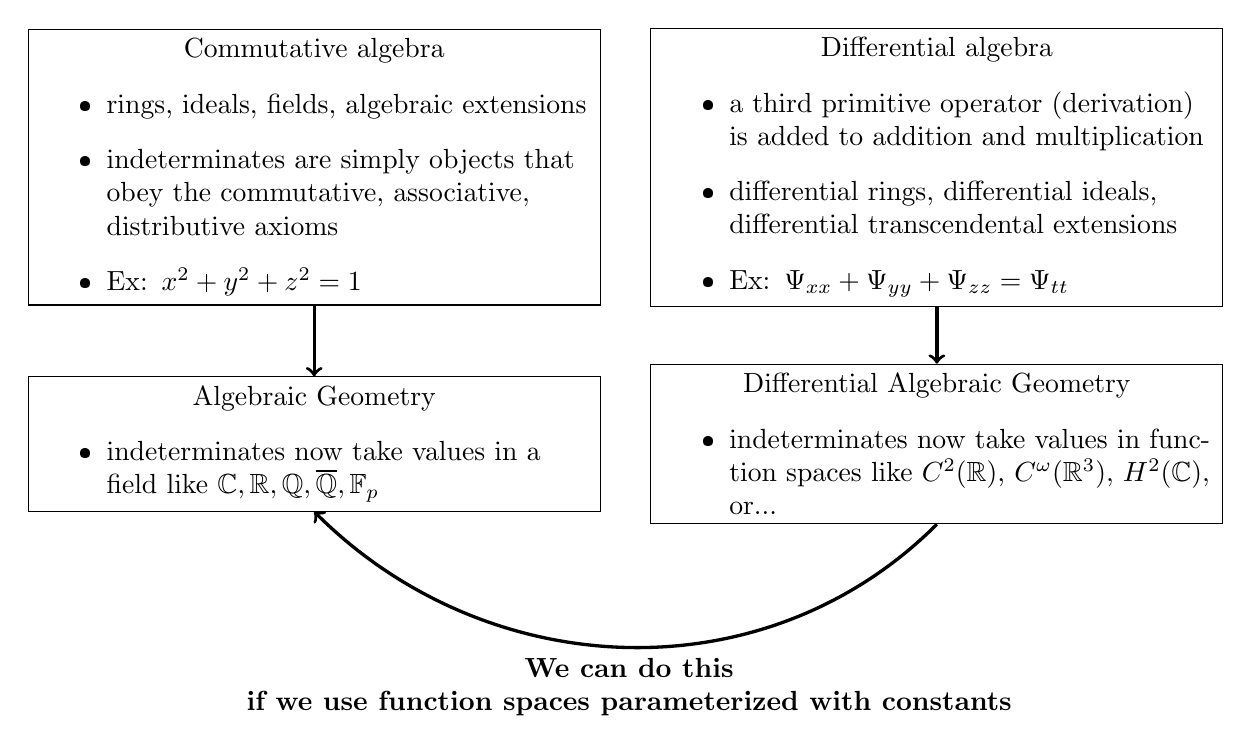
\begin{tikzpicture}[node distance=50pt, every text node part/.style={align=center}]
\node (commutative algebra) [draw, text width=200pt] {Commutative algebra
      \begin{itemize}
        \item rings, ideals, fields, algebraic extensions
        \item indeterminates are simply objects that obey the commutative, associative, distributive axioms
        \item Ex: $x^2+y^2+z^2=1$
      \end{itemize}
};
\node (algebraic geometry) [draw, node distance=100pt, below of=commutative algebra, text width=200pt] {Algebraic Geometry
      \begin{itemize}
        \item indeterminates now take values in a field like $\mathbb{C}, \mathbb{R}, \mathbb{Q}, \overline{\mathbb{Q}}, \mathbb{F}_p$
      \end{itemize}
};
\node (differential algebra) [draw, node distance=225pt, right of=commutative algebra, text width=200pt] {Differential algebra
      \begin{itemize}
        \item a third primitive operator (derivation) is added to addition and multiplication
        \item differential rings, differential ideals, differential transcendental extensions
        \item Ex: $\Psi_{xx}+\Psi_{yy}+\Psi_{zz}=\Psi_{tt}$
      \end{itemize}
};
\node (differential algebraic geometry) [draw, node distance=100pt, below of=differential algebra, text width=200pt] {Differential Algebraic Geometry
      \begin{itemize}
        \item indeterminates now take values in function spaces like $C^2(\mathbb{R})$,
$C^\omega(\mathbb{R}^3)$, $H^2(\mathbb{C})$, or...
      \end{itemize}
};

\draw [very thick, ->] (commutative algebra.south) -- (algebraic geometry.north);
\draw [very thick, ->] (differential algebra.south) -- (differential algebraic geometry.north);

\draw [very thick, ->] (differential algebraic geometry.south) to[out=-135, in=-45] (algebraic geometry.south);

\node at (4,-6.6) {\bf We can do this\\\bf if we use function spaces parameterized with constants};

\end{tikzpicture}%
}
\end{figure}

%What kind of reduction step

%Practical experience with this algorithm suggests that, given the current
%state of software development, it is best to use a slightly inferior
%variant of this algorithm, where a standard Gr\"obner basis algorithm
%is used instead of Rosenfeld-Gr\"obner.  Considering that Rosenfeld-Gr\"obner
%is a generalization of Buchberger's algorithm, and given the computational
%complexity of computing a Gr\"obner basis, it makes sense to use
%existing Gr\"obner basis software, hoping that in the future, we
%will have a comprehensive Rosenfeld-Gr\"obner implementation that
%will handle differential polynomials as well as conventional polynomials,
%incorporate all the fruits of
%our research into the computation of Gr\"obner bases,
%and fall back into an efficient Gr\"obner basis calculation
%when presented with the degenerate case of a system of polynomial equations.

%We can describe a slightly inferior variant of this algorithm, that only
%requires the calculation of Gr\"obner bases to complete a primary decomposition.
%utility of algebraic geometry in the differential algebra setting by parameterizing
%the function space using only a finite number of constants, and doing so in such
%a way that the constants can be isolated into a system of polynomial equations,
%which can then be solving using algebraic geometry.

%What specific restrictions must be imposed to acheive this?

%  - new indeterminants must be specified as ODEs
%  - we need to cancel the leading derivative

%If, for example, we expect
%our solution to be in $C^2(\mathbf{R})$, then we parameterize a subset of
%$C^2(\mathbb{R})$ using some number of complex variables, say twenty, so that our resulting
%equations are polynomials in $\mathbb{C}[c_0,..,c_{19}]$ and their common
%solutions describe an algebraic variety in $\mathbb{C}^{20}$.
%Unfortunately, degree bounds seem necessary on almost everything in order
%to achieve this, and no matter how big and complicated our equations become,
%we're only searching part of the function space.

%An algorithm begins to suggest itself.  We can recover the
%utility of algebraic geometry in the differential algebra setting by parameterizing
%the function field using only a finite number of constants, and doing so in such
%a way that the constants can be isolated into a system of polynomial equations,
%which can then be solving using algebraic geometry.  If, for example, we expect
%our solution to be in $C^2(\mathbb{R})$, then we parameterize a subset of
%$C^2(\mathbb{R})$ using some number of complex variables, say twenty, so that our resulting
%equations are polynomials in $\mathbb{C}[c_0,..,c_{19}]$ and their common
%solutions describe an algebraic variety in $\mathbb{C}^{20}$.
%Unfortunately, degree bounds seem necessary on almost everything in order
%to achieve this, and no matter how big and complicated our equations become,
%we're only searching part of the function space.

In short, rather than attempt to derive differential equations that apply to all solutions
of the PDE, we restrict our attention to an {\bf ansatz}, a subset of the function
space in which we seek solutions, parameterized as a finite dimensional vector space over the constants.
If we can, by luck or by theory, pick a good ansatz, then we have
a computable algorithm to find the solutions therein.

\subsection*{The Ansatz}

These are the primary requirements
for an {\bf ansatz}:

\begin{itemize}
%% \item it must be formed from a finite sequence of linear ODE and algebraic extensions, and
\item it expresses a restricted form for the solution to the PDE
\item it must be expressed using differential polynomials,
\item it may involve additional indeterminates, which may or may not be constants
\end{itemize}

%Additionally, I am specifically looking for solutions that can be constructed using ODEs.
One of the most fundamental questions to ask of a PDE is whether can it
be solved using ODEs.  We can't definitely answer this question using
this algorithm, but as these are the types of solutions I am interested in,
all of the current ansatzen attempt to express solutions to the PDE using
a finite number of ODEs.

Futhermore, I restrict to homogeneous linear ODEs,
%first because their theory and practice is more refined, and second
because the PDEs I am primarily interested in solving (various forms of Schr\"odinger's equation)
are homogeneous and linear, so I'm hopeful that homogeneous linear ODEs will suffice to solve them.
This is not a fundamental requirement or limitation of the algorithm.

A $n^{\rm th}$-order homogeneous linear ODE takes the form:

\begin{equation}
a_n(v) y^{(n)} + a_{n-1}(v) y^{(n-1)} \cdots a_1(v) y' + a_0(v) y = 0
\end{equation}

where $y^{(n)}, y^{(n-1)}, ... y'$ are derivatives of the dependent variable $y$ with respect to the independent variable $v$.

% How to introduce a new ODE?  First, we wish to avoid the complexities of introducing new derivations,
% so we seek to specify how the ODE behaves under the existing derivations.

We introduce the dependent variable $y$ by adjoining a new indeterminant that is defined using a differential polynomial
whose coefficients are all univariate functions of a single {\it independent variable} $v$,
and whose derivatives, at least conceptionally, are all taken with respect to that
independent variable.  This independent variable $v$ is also a new indeterminant,
selected from the underlying field and itself parameterized by constants,
which is expressed using a simple equality between the new indeterminant $v$ and its parameterized form.

The coefficients of the ODE's defining differential polynomial are
selected not from the existing field, but rather from ${\mathbb Q}(v)$, an auxiliary field
constructed using the distinguished variable $v$.
We could also consider coefficients selected from an extension
of ${\mathbb Q}(v)$, but that is not required for the present work.

Example: Over the rational function field $\mathbb{C}(x)$, we can construct an ODE
extension specified by the primitive element $\Psi$, minimial differential polynomial
$\Psi' = \Psi$, and distinguished variable $v$, which we equate to $x+r$.  This is a differential polynomial
that maps to the analytic equation $\frac{d\Psi}{dv}=\Psi$ and is solved
by the analytic functions $Ae^v$ ($A$ is an arbitrary constant).  Substituting in $v=x+r$, we see that
the functions $Ae^{x+r}$ are solutions to this ODE extension.

I use apostrophes, and not the jet notation subscripts, when writing
the differential polynomial in the ODE case to emphasize that we are not introducing a new derivation,
nor is the ODE's derivative any of the existing derivations.

How can derivations with respect to a new variable be connected with the existing derivations?
We can expess our previously existing derivations in terms of the new one using the chain rule.
In fact, all that required is to specify how the new interderminates behave under the existing
derivations, and that relationship is simply ${\rm d}\Psi/{\rm d}x = {\rm d}\Psi/{\rm d}v\cdot {\rm d}v/{\rm d}x$

In short, to introduce a new ODE (second-order, for the purposes of illustration):

\begin{itemize}
% \item We wish to avoid introducing new derivations.
\item We introduce new indeterminates $\Psi$, $\Psi'$, $\Psi'', v$
\item We introduce a new differential polynomial involving only $\Psi''$, $\Psi'$, $\Psi$, $v$, and constants,
and using no non-constant indeterminates or existing derivations
\item We define the derivations of $\Psi$ and $\Psi'$ using the chain rule: \break $\Psi_x = \Psi' v_x$; $\Psi'_x = \Psi'' v_x$
\item We equate the independent variable $v$ to some parameterized differential polynomial
\end{itemize}

All derivations of $\Psi''$ are now completely defined by these differential polynomials.
%(assuming that polynomial is first degree in $\Psi''$, and its initial involves only $v$)
%(the derivations would be defined even without this restriction, but might involve $\Psi''$ itself)
%(the assumption allows $\Psi''$ to eliminated by differential reduction)

\tikzstyle{poly}=[rectangle, draw, thick, fill=white, text width=5em, align=center, rounded corners, minimum height=2em]
\tikzstyle{poly2}=[rectangle, draw, thick, fill=white, align=center, rounded corners, minimum height=2em]
\tikzstyle{ring}=[rectangle, draw=blue, thick, fill=blue!20, text width=5em,align=center, rounded corners, minimum height=2em]
\tikzstyle{element}=[rectangle, draw=orange, thick, fill=orange!20, align=center, rounded corners, minimum height=2em]
\tikzstyle{algebraic}=[rectangle, draw=green, thick, fill=green!20, align=center, rounded corners, minimum height=2em]
\tikzstyle{degree}=[]

%% {\bf Ansatz 5}

\begin{figure}
\centering
  \begin{tikzpicture}[remember picture,out=315,in=225,distance=0.4cm,node distance=40pt]
    \node (Psi) [poly, text width=100pt] {$\framebox(10,10){}\tikzmark{a}\,\Psi'' + \framebox(10,10){}\tikzmark{b}\,\Psi' + \coeff\tikzmark{c}\,\Psi$};
    \node (Qv) [ring, below of=Psi, text width=100pt] {$\mathbb{Q}[v]$};
    \node (v) [poly, right=of Qv] {$v$};
    \draw[degree] (a.west) -- (a.west|-Qv.north) node[right,pos=0.6] {1};
    \draw[degree] (b.west) -- (b.west|-Qv.north) node[right,pos=0.6] {1};
    \draw[degree] (c.west) -- (c.west|-Qv.north) node[right,pos=0.6] {1};
    \node (Psi label) [at=(v.east|-Psi.north), anchor=north east] {\Large$\Psi$};
    \begin{scope}[on background layer]
        \node (Psi block)[fit=(Psi) (Qv) (v), inner sep=10pt, element] {};
    \end{scope}
    \node (base) [ring, node distance=70pt, below=of Psi block.east, anchor=east, text width=250pt] {$\mathbb{Q}[x,y,z,r]/(r^2-x^2-y^2-z^2)$};
    \draw[degree] (v.south) -- (v.south|-base.north) node[right,pos=0.7] {1};
  \end{tikzpicture}
\end{figure}

For example, consider the ansatz formed from 
a second-order ODE element with first-degree coefficients and a distinguished variable formed
as a first-degree polynomial in the underlying differential polynomial ring.
See figure 2, where polynomial degrees are signified by the black numbers next to the lines connecting them to the rings they are selected from.
%Note in particular that there is no green box around the orange one.  The ODE
%element must itself solve the PDE; we do not construct the full extension field it would naturally generate.
We do not construct any more complicated function from $\Psi$ (although we could);
the element $\Psi$ must itself solve the PDE.

The structure of this ansatz is described using differential polynomials as follows.

A differential polynomial involving only $\Psi''$, $\Psi'$, $\Psi$, $v$, and constants,
and using no non-constant indeterminates or existing derivations:

\begin{equation}
\label{ansatz 5b}
(a_0 + a_1 v) \Psi'' + (b_0 + b_1 v) \Psi' + (c_0 + c_1 v) \Psi = 0 \\
\end{equation}

The derivations of $\Psi$ and $\Psi'$, defined using the chain rule:

\begin{equation}
\label{ansatz 5c}
\begin{gathered}
\Psi_x = \Psi' v_x \qquad
\Psi_y = \Psi' v_y \qquad
\Psi_z = \Psi' v_z \\
\Psi'_x = \Psi'' v_x \qquad
\Psi'_y = \Psi'' v_y \qquad
\Psi'_z = \Psi'' v_z \\
\end{gathered}
\end{equation}

The distinguished variable $v$:

\begin{equation}
\label{ansatz 5a}
v = v_1 x + v_2 y + v_3 z + v_4 r
\end{equation}

Our differential ring is equipped with three derivations $x$, $y$, and $z$
(this is not apparent in the graphical representation).  Our base ring
is $\mathbb{Q}[x,y,z,r]/(r^2-x^2-y^2-z^2)$, and from this we select
a linear variable $v$ using equation \eqref{ansatz 5a}.
The $v_i$'s (and the $a_i$'s, $b_i$'s and $c_i$'s) are constants.
Strictly speaking, a $v_0$ constant term
should also be present, but I often drop the constant term from the
distinguished variable of an ODE extension, because taking
the derivative with respect to $x+3$ is no different from taking
the derivative with respect to $x$.

Next we introduce our new ODE element $\Psi$, which will
also be the solution to our PDE.
We now wish to essentially introduce a new derivation with respect to $v$.
While I could write $\Psi_v$, I do not wish to confuse this derivation
with the existing three derivations, plus I wish to emphasis
that we don't need to actually introduce any new derivations,
so I'll write this as $\Psi'$.  Treat $\Psi$, $\Psi'$, and
$\Psi''$ as new indeterminates.
$\Psi$ must satisfy the minimial differential polynomial, which
we specify in equation \eqref{ansatz 5b}, also introducing
degree bounds on the coefficients.

Finally, we need to connect our new derivation with the existing derivations.
Equations \eqref{ansatz 5c} show how to evaluate
the derivatives of $\Psi$ and $\Psi'$ with respect to the
existing derivations in the differential ring (it's just the chain rule).
Although conceptually we introduce another derivation, it is important
to note that we do not have to add any new derivations to the original differential ring.
All that is needed is
to add $\Psi$, $\Psi'$, and $\Psi''$ as new indeterminates
and specify how they behave with respect to the existing derivations.

\subsection*{Differential Reduction}

Having defined an ansatz, we now use it to reduce our original PDE.  For this purpose,
we use Ritt's full reduction algorithm; see \cite{Ritt} Chapter I, \S 6 or \cite{Kolchin}, Chapter I, \S 9.
A compact description of the relevant concepts can be found in Section 3 of \cite{blop}.
A comparison of various techniques used to solve systems of polynomial and differential polynomial equations can be found in \cite{aistleitner}.

We define a ranking on the indeterminants and their derivations, which is a distinct concept from an ordering on the monomials, as used,
for example, in defining a Gr\"obner basis.  We
define the {\it leader} of a polynomial as the highest ranking indeterminant that appears in the polynomial.

To reduce a differential polynomial $p$ by a system $S$ of differential polynomials,
we see if there exists a polynomial in $S$ any higher derivative of the leader of a polynomial in $S$ appears in $p$.
If so, we pick the highest ranking

[describe Ritt's algorithm]

\subsection*{Projection}

Having defined an ansatz and used it to reduce the original PDE, we now project
that reduced equation into the solution space of the constants.  We do this
by factoring each polynomial term into its constant and non-constant indeterminants,
and gathering together like terms with identical non-constant factors.  Setting the
constant coefficients of each term to zero produces a system of polynomial equations,
involving only the constants, that will solve the original PDE when satisfied.

This system of equations defines an algebraic variety, but it need not be irreducible.
Several algorithms have been proposed and implemented to decompose an algebraic
variety into its irreducible components.

\begin{comment}
Any particular selection of constants produces a system of differential polynomials that defines a differential ideal.

Which of those differential ideals reduce the original PDE to zero?

i.e, I^i S^s PDE = [A]

(A, I, and S are parameterized by constants)

if all of the A's are equal to zero, then either the PDE is equal to zero or one of the I's and/or S's is equal to zero

for some selection of the constants, this creates a specific A, I, and S.  Q: does this solve the PDE?
   what does this question mean?
   does setting all of the A's to zero (i.e, make them all true) imply that the PDE is zero?
   it implies that either the PDE is zero, or an I/S is zero

in my case, I'm ``ignoring the denominator'', meaning that I'm ignoring I and S.  If I or S were to be zero,
then the PDE would not have to be zero, i.e, would not have to be satisfied

So, we want to check that the ``denominator'' (I and S) is not zero.  If they were, the PDE might not be satisfied.

If an I or an S is zero, then we could add it to the system and check again

For any solution in the variety of the constants, if I/S is zero, then it might not solve the PDE.
Q: what do we do then?

Q: if some selection of constants solves the PDE, do we always find it using this algorithm?
\end{comment}

\subsection*{Solution Algorithm}

To summarize, given a PDE defined by one or more differential polynomials, do the following:

\begin{enumerate}
\item Select an ansatz that defines a differential function space parameterized by constants

\item Reduce the PDE modulo the ansatz (differential elimination step)

\item Construct a system of polynomial equations in the constants by collecting like terms in the remaining variables (projection step)

\item Form a polynomial ideal from that system of equations, and compute its associated prime ideals

\item Each prime ideal corresponds to a variety in the vector space of constants,
the union of which form the solution space of the PDE in the differential function space

\end{enumerate}

%%\section*{An Example: The New Solution of Hydrogen}
\subsection*{An Example: A New Pseudo-Solution of Hydrogen}

We seek to demonstrate the operation of the algorithm on the following Schr\"odinger equation for hydrogen:

\begin{equation}
\label{schrodinger hydrogen}
-\frac{1}{2}\nabla^2 \Psi - \frac{1}{r}\Psi = E \Psi
\end{equation}

where $\nabla$ is the Laplacian, $\Psi$ is a complex-valued wavefunction defined over real 3-dimensional space,
and $r$ is the distance to the origin.  We choose to work in Cartesian coordinates, so $r^2=x^2+y^2+z^2$,
and use Hartree atomic units to render the equation dimensionless, though for our purposes we can
ignore any physical interpretation of the problem and treat it simply as an equation to be solved.

We'll use the ansatz from the previous section, a second-order ODE with linear coefficients and a linear distinguished variable, i.e:

\begin{center}
  \begin{tikzpicture}[remember picture,out=315,in=225,distance=0.4cm,node distance=40pt]
    \node (Psi) [poly, text width=100pt] {$\framebox(10,10){}\tikzmark{a}\,\Psi'' + \framebox(10,10){}\tikzmark{b}\,\Psi' + \coeff\tikzmark{c}\,\Psi$};
    \node (Qv) [ring, below of=Psi, text width=100pt] {$\mathbb{Q}[v]$};
    \node (v) [poly, right=of Qv] {$v$};
    \draw[degree] (a.west) -- (a.west|-Qv.north) node[right,pos=0.6] {1};
    \draw[degree] (b.west) -- (b.west|-Qv.north) node[right,pos=0.6] {1};
    \draw[degree] (c.west) -- (c.west|-Qv.north) node[right,pos=0.6] {1};
    \node (Psi label) [at=(v.east|-Psi.north), anchor=north east] {\Large$\Psi$};
    \begin{scope}[on background layer]
        \node (Psi block)[fit=(Psi) (Qv) (v), inner sep=10pt, element] {};
    \end{scope}
    \node (base) [ring, node distance=70pt, below=of Psi block.east, anchor=east, text width=250pt] {$\mathbb{Q}[x,y,z,r]/(r^2-x^2-y^2-z^2)$};
    \draw[degree] (v.south) -- (v.south|-base.north) node[right,pos=0.7] {1};
  \end{tikzpicture}
\end{center}

\begin{equation}
\label{ansatz 5}
\begin{gathered}
\begin{comment}
\Psi_x = \frac{\Psi'}{v_x} \qquad
\Psi_y = \frac{\Psi'}{v_y} \qquad
\Psi_z = \frac{\Psi'}{v_z} \\
\Psi'_x = \frac{\Psi''}{v_x} \qquad
\Psi'_y = \frac{\Psi''}{v_y} \qquad
\Psi'_z = \frac{\Psi''}{v_z} \\
\end{comment}
\Psi_x = \Psi' v_x \qquad
\Psi_y = \Psi' v_y \qquad
\Psi_z = \Psi' v_z \\
\Psi'_x = \Psi'' v_x \qquad
\Psi'_y = \Psi'' v_y \qquad
\Psi'_z = \Psi'' v_z \\
(a_0 + a_1 v) \Psi'' + (b_0 + b_1 v) \Psi' + (c_0 + c_1 v) \Psi = 0 \\
v = v_1 x + v_2 y + v_3 z + v_4 r
\end{gathered}
\end{equation}

\subsection*{Differential Reduction Step}

%I attempted to use the Rosenfeld-Gr\"obner algorithm to reduce equation \eqref{schrodinger hydrogen}
%modulo \eqref{ansatz 5}, but it ultimately ran out of memory on a 96 GB computer after
%30 hours.  Instead, I used Sage to construct a polynomial ring modulo the ideal
%$r^2-x^2-y^2-z^2$ to handle the algebraic extension (present not in the ansatz proper,
%but in the original ring used to construct the PDE).  Next I directed the software
%to expand the derivatives in \eqref{schrodinger hydrogen} and substitute for $\Psi''$ and $v$
%according to the ansatz \eqref{ansatz 5}.  The result is
%a rational function
%with a 228 term numerator and an 18 term denominator.  We ignore the denominator.  The numerator begins:

To \eqref{ansatz 5} I appended
$r^2-x^2-y^2-z^2$ to handle the algebraic extension used
in the underlying polynomial ring to construct the PDE, and obtained
the following system of differential polynomials:

\begin{equation}
\label{ansatz 5 plus}
\begin{gathered}
\begin{comment}
\Psi_x = \frac{\Psi'}{v_x} \qquad
\Psi_y = \frac{\Psi'}{v_y} \qquad
\Psi_z = \frac{\Psi'}{v_z} \\
\Psi'_x = \frac{\Psi''}{v_x} \qquad
\Psi'_y = \frac{\Psi''}{v_y} \qquad
\Psi'_z = \frac{\Psi''}{v_z} \\
\end{comment}
\Psi_x = \Psi' v_x \qquad
\Psi_y = \Psi' v_y \qquad
\Psi_z = \Psi' v_z \\
\Psi'_x = \Psi'' v_x \qquad
\Psi'_y = \Psi'' v_y \qquad
\Psi'_z = \Psi'' v_z \\
(a_0 + a_1 v) \Psi'' + (b_0 + b_1 v) \Psi' + (c_0 + c_1 v) \Psi = 0 \\
v = v_1 x + v_2 y + v_3 z + v_4 r \\
r^2-x^2-y^2-z^2
\end{gathered}
\end{equation}

\eqref{ansatz 5 plus} (ordering? also, they're equations, not polynomials) is a differentially triangular system, although this property
is not required to ensure the correct operation of the algorithm.  Next, I used Sage,
along with some additional Python code, to differentially reduce \eqref{schrodinger hydrogen}
modulo \eqref{ansatz 5 plus}, using Ritt's reduction algorithm.
The result is a rational function
with a 228 term numerator and an 18 term denominator.  The numerator begins:

% I used a Sage-based computer program with the following ansatz.
\begin{comment}
I found this solution roughly as follows.\footnote{
I discovered an alternate form of this solution using a somewhat more complex ansatz
on January 24, 2023.  By January 26, I had established the solution in its current form.
The original ansatz produced a rational function with
a 1254 term numerator and a 36 term denominator, that gave rise to a system of 224 equations,
and was first solved using numerical approximation (scipy.optimize.root).
}

Use Cartesian coordinates.  Let $v$ be a linear polynomial in the coordinates and the root $r=\sqrt{x^2+y^2+z^2}$,
Reduce the input PDE \eqref{schrodinger} modulo differential ideal \eqref{ansatz 5}, obtaining
\end{comment}

\begin{equation}
\label{schrodinger modulo ansatz 5}
%sage: print(latex(sum(eq_a_reduceRing_n.terms()[0:4])).replace('Zeta', 'Psi'))
% then add "+ \cdots" at the end
r \Psi' x^{3} v_{1}^{3} b_{1} + r \Psi' x y^{2} v_{1}^{3} b_{1} + r \Psi' x z^{2} v_{1}^{3} b_{1} + r \Psi' x^{2} y v_{1}^{2} v_{2} b_{1} + \cdots
\end{equation}

The denominator, after replacing $x^2+y^2+z^2$ with $r^2$, reads:

\begin{equation}
2 r^3 (a_1 (v_1 x + v_2 y + v_3 z + v_4 r) + a_0)
\end{equation}

Ordering: right now, we use term ordering with lex(r) then degrevlex on the rest, so our terms are ordered first by $r$,
then degrevlex.  But I'm collecting terms (in build\_system\_of\_equations) by looping over the numerator and
collecting like terms.  Note that the first four terms above were ordered using the term ordering.



\subsection*{Projection Step}

Having reduced our PDE \eqref{schrodinger hydrogen} by the differential ideal defined by \eqref{ansatz 5},
we now wish to project our solution into the vector space of the constants.  We're looking for
constants that will solve equation \eqref{schrodinger modulo ansatz 5} for all values of $x$, $y$, $z$, $r$,
$\Psi$, and $\Psi'$, so
we collect like terms in $x$, $y$, $z$, $r$, $\Psi$, and $\Psi'$, organizing the numerator like this:

\begin{equation}
%sage: print(latex(Factorization([(e,1) for e in list(system_of_like_terms.items())[0]], sort=False)).replace('Zeta','Psi'))
%(r \Psi' x^{3}) \cdot (v_{1}^{3} b_{1} + v_{1} v_{2}^{2} b_{1} + v_{1} v_{3}^{2} b_{1} + 3 v_{1} v_{4}^{2} b_{1})
% then drop the parens and the \cdot and add plus sign and \cdots at the end
r \Psi' x^{3} (v_{1}^{3} b_{1} + v_{1} v_{2}^{2} b_{1} + v_{1} v_{3}^{2} b_{1} + 3 v_{1} v_{4}^{2} b_{1}) + \cdots
\end{equation}

The expressions in parenthesis gives us a system of equations (only one is shown)
involving only constants
that, if satisfied,
will yield a solution to \eqref{schrodinger hydrogen} in the form \eqref{ansatz 5}.  Once
duplicate equations are dropped, the system has 34 equations.  Note that $E$, although
not a parameter in the ansatz, is included with them because it is a constant.  The
correct operation of the algorithm is predicated on nothing more than separating
the indeterminants into constants and non-constants, and it makes no difference whether
the constants are introduced in the ansatz or appear in the original PDE.

%%sage: latex(matrix(eqns()).transpose())
%% The problem with making this a "figure" is that it's a numbered system of equations
%%\begin{figure}
\begin{equation}
\label{polynomial system}
% sage: latex(matrix(eqns_RQQ).transpose())
% then remove \left( and \right)
\begin{array}{r}
4 v_{1} v_{3} v_{4} b_{1} \\
v_{1}^{2} v_{2} b_{1} + v_{2}^{3} b_{1} + v_{2} v_{3}^{2} b_{1} + 3 v_{2} v_{4}^{2} b_{1} \\
-2 v_{4} a_{0} \\
4 v_{1}^{2} v_{4} b_{1} + 4 v_{2}^{2} v_{4} b_{1} + 2 v_{3}^{2} v_{4} b_{1} + 2 v_{4}^{3} b_{1} \\
3 v_{1}^{2} v_{4} b_{1} + v_{2}^{2} v_{4} b_{1} + v_{3}^{2} v_{4} b_{1} + v_{4}^{3} b_{1} \\
v_{1}^{2} v_{3} b_{1} + v_{2}^{2} v_{3} b_{1} + v_{3}^{3} b_{1} + 3 v_{3} v_{4}^{2} b_{1} \\
2 v_{1}^{2} v_{4} c_{1} + 4 v_{2}^{2} v_{4} c_{1} + 4 v_{3}^{2} v_{4} c_{1} + 2 v_{4}^{3} c_{1} - 4 E v_{4} a_{1} \\
4 v_{1} v_{3} v_{4} c_{1} \\
v_{1}^{2} v_{3} c_{1} + v_{2}^{2} v_{3} c_{1} + v_{3}^{3} c_{1} + 3 v_{3} v_{4}^{2} c_{1} - 2 E v_{3} a_{1} \\
2 v_{2} v_{4} c_{0} - 2 v_{2} a_{1} \\
-2 v_{2} v_{4} a_{1} + 2 v_{2} v_{4} b_{0} \\
4 v_{1}^{2} v_{4} c_{1} + 4 v_{2}^{2} v_{4} c_{1} + 2 v_{3}^{2} v_{4} c_{1} + 2 v_{4}^{3} c_{1} - 4 E v_{4} a_{1} \\
3 v_{1}^{2} v_{4} c_{1} + v_{2}^{2} v_{4} c_{1} + v_{3}^{2} v_{4} c_{1} + v_{4}^{3} c_{1} - 2 E v_{4} a_{1} \\
v_{1}^{2} v_{4} c_{1} + 3 v_{2}^{2} v_{4} c_{1} + v_{3}^{2} v_{4} c_{1} + v_{4}^{3} c_{1} - 2 E v_{4} a_{1} \\
4 v_{1}^{2} v_{4} c_{1} + 2 v_{2}^{2} v_{4} c_{1} + 4 v_{3}^{2} v_{4} c_{1} + 2 v_{4}^{3} c_{1} - 4 E v_{4} a_{1} \\
4 v_{2} v_{3} v_{4} c_{1} \\
v_{1}^{2} v_{4} c_{1} + v_{2}^{2} v_{4} c_{1} + 3 v_{3}^{2} v_{4} c_{1} + v_{4}^{3} c_{1} - 2 E v_{4} a_{1} \\
2 v_{3} v_{4} c_{0} - 2 v_{3} a_{1} \\
-2 a_{0} \\
-2 v_{4}^{2} a_{1} + v_{1}^{2} b_{0} + v_{2}^{2} b_{0} + v_{3}^{2} b_{0} + v_{4}^{2} b_{0} \\
2 v_{1}^{2} v_{4} b_{1} + 4 v_{2}^{2} v_{4} b_{1} + 4 v_{3}^{2} v_{4} b_{1} + 2 v_{4}^{3} b_{1} \\
v_{1}^{2} v_{4} b_{1} + v_{2}^{2} v_{4} b_{1} + 3 v_{3}^{2} v_{4} b_{1} + v_{4}^{3} b_{1} \\
4 v_{1} v_{2} v_{4} c_{1} \\
v_{1}^{3} b_{1} + v_{1} v_{2}^{2} b_{1} + v_{1} v_{3}^{2} b_{1} + 3 v_{1} v_{4}^{2} b_{1} \\
-2 v_{3} v_{4} a_{1} + 2 v_{3} v_{4} b_{0} \\
v_{1}^{2} c_{0} + v_{2}^{2} c_{0} + v_{3}^{2} c_{0} + v_{4}^{2} c_{0} - 2 E a_{0} - 2 v_{4} a_{1} \\
2 v_{1} v_{4} c_{0} - 2 v_{1} a_{1} \\
v_{1}^{2} v_{2} c_{1} + v_{2}^{3} c_{1} + v_{2} v_{3}^{2} c_{1} + 3 v_{2} v_{4}^{2} c_{1} - 2 E v_{2} a_{1} \\
-2 v_{1} v_{4} a_{1} + 2 v_{1} v_{4} b_{0} \\
v_{1}^{2} v_{4} b_{1} + 3 v_{2}^{2} v_{4} b_{1} + v_{3}^{2} v_{4} b_{1} + v_{4}^{3} b_{1} \\
v_{1}^{3} c_{1} + v_{1} v_{2}^{2} c_{1} + v_{1} v_{3}^{2} c_{1} + 3 v_{1} v_{4}^{2} c_{1} - 2 E v_{1} a_{1} \\
4 v_{1} v_{2} v_{4} b_{1} \\
4 v_{1}^{2} v_{4} b_{1} + 2 v_{2}^{2} v_{4} b_{1} + 4 v_{3}^{2} v_{4} b_{1} + 2 v_{4}^{3} b_{1} \\
4 v_{2} v_{3} v_{4} b_{1}
\end{array}
\end{equation}
%% \end{figure}

\subsection*{Prime Decomposition}

\begin{comment}
I used a numerical algorithm to solve the system of equations in expectation
of it being faster for larger systems, but the system \eqref{polynomial system}
is small enough that exact methods are usable.
\end{comment}
We now form
an ideal $I$ in $\mathbb{Q}[v_0,...,m_1,E]$ from \eqref{polynomial system}, and
seek to compute its associated prime ideals.

%Sage can calculate a Gr\"obner basis for the radical $I$ in less than a second.
%While we could work with the Gr\"obner basis directly\footnote{A Gr\"obner basis
%of the solution ideal in lexicographic order $E>d_i>m_i>n_i>v_i$ contains 65 polynomials.}
%, I find it more
%useful to study the primary decomposition, which Sage computes using
%the Shimoyama-Yokoyama algorithm\footnote{Localization and Primary Decomposition of
%Polynomial Ideals, {\it J. Symbolic Computation} (1996) {\bf 22}, 247–277}
%as implemented in Singular.  Gr\"obner basis calculations are done
%as a subalgorithm of Shimoyama-Yokoyama.

Taking the radical of the ideal simplifies both the theory and the application,
and can be justified because there are no nilpotent elements in our solution
space, which is just 11-dimensional complex space ${\mathbb C}^{11}$.  The
primary decomposition of a radical ideal is also a prime decomposition,
as the distinction between primary and prime ideals is only significant
for non-radical ideals with nilpotent elements.  Sage/Singular computes
the following decomposition into prime ideals:

\begin{verbatim}
sage: I.radical().primary_decomposition()
\end{verbatim}

\newcommand{\Bold}[1]{\mathbb{#1}}

\begin{subequations}
\label{ideal}
%sage: latex(I.minimal_associated_primes())
\begin{align}
% sage: sorted([latex(tuple(P.gens())) for P in I.minimal_associated_primes()])
% remove the list brackets and commas, add & at the beginning of each line, add \label and \\ at end of each line, normalize a fraction
& \left(a_{0}, v_{4}, v_{3}, v_{2}, v_{1}\right)\label{ideal:5} \\
& \left(c_{1}, c_{0}, b_{1}, b_{0}, a_{1}, a_{0}\right)\label{ideal:4} \\
& \left(v_{1}^{2} + v_{2}^{2} + v_{3}^{2}, a_{1}, a_{0}, v_{4}\right)\label{ideal:3} \\
& \left(v_{4} c_{0} - b_{0}, E c_{0} - v_{4} c_{1}, -v_{4}^{2} c_{1} + E b_{0}, b_{1}, 2 a_{1} - b_{0}, a_{0}, v_{3}, v_{2}, v_{1}\right)\label{ideal:2} \\
& \left(v_{4} c_{0} - b_{0}, v_{1}^{2} + v_{2}^{2} + v_{3}^{2} - v_{4}^{2}, c_{1}, b_{1}, a_{1} - b_{0}, a_{0}, E\right)\label{ideal:1}
\end{align}
\end{subequations}

Several of these varieties solve the system of equations, but do not lead to a meaningful solution to the differential equation.
In brief,

\begin{itemize}
\item[\eqref{ideal:5}] sets the variable $v$ to zero, so we discard it,
\item[\eqref{ideal:4}] sets all coefficients of the ODE to zero, so we discard it,
\item[\eqref{ideal:3}] sets the coefficient of
%$\frac{d^2\Psi}{dv^2}$
%$D^2\Psi$
$\Psi''$
in the ODE to zero, resulting in a first-order ODE, so we discard it, too,
\item[\eqref{ideal:2}] corresponds to the classical solutions (see below), and
\item[\eqref{ideal:1}] gives us our new solution (see below).

\end{itemize}

How to understand ideal \eqref{ideal:2}?  $a_0$ is an ideal generator,
so $a_0=0$, and we can always multiply our homogenous differential polynomial by a constant without affecting our result, so we can set $a_1=1$.
Likewise, we can multiply our variable $v$ by a constant and that will only change our coefficients by constants,
and $v_1=v_2=v_3=0$, so we can normalize by setting $v_4=1$.  This immediately implies that $b_0 = c_0 = 2$ and simplifies ideal \eqref{ideal:2} to:

\begin{equation}
\left(v_{3}, v_{2}, v_{1}, v_{4} - 1, c_{0} - 2, 2 E - c_{1}, b_{1}, 2 - b_{0}, a_{1} - 1, a_{0}\right)
\end{equation}

\begin{equation}
\label{classical eq in ideal}
\begin{gathered}
v=r \\
v \Psi'' + 2 \Psi' + 2(1 + E v) \Psi = 0
\end{gathered}
\end{equation}

This is the classical radial equation obtained by seperation of variables\footnote{See
Pauling and Wilson or
\url{http://hyperphysics.phy-astr.gsu.edu/hbase/quantum/hydrad.html}}.  We use
spherical coordinates, set $\Psi = R(r)P(\theta)F(\psi)$, and obtain the above equation for $R(r)$,
though it is more commonly written in this form:

\begin{equation}
\frac{1}{R} \frac{d}{dr}\left[ r^2 \frac{dR}{dr}\right] + 2(Er^2 + r) = l(l+1)
\end{equation}

where $l$ is the orbital quantum number, which can be zero.  Set $l=0$, $v=r$ and $\Psi=R$ and
expand out the derivative to obtain \eqref{classical eq in ideal}.  This solution has been
known for a hundred years; its presence here was expected and won't be commented on further.

Ideal \eqref{ideal:1} was not expected, and contains our new solution.
$a_0$ is an ideal generator,
so $a_0=0$, and we can set $a_1=1$, by the same logic as above.
If we limit our $v_i$ coefficients to be real, all of their squares must
be positive, and since $v_1^2+v_2^2+v_3^3-v_4^2=0$, $v_4$ must be non-zero.  So we can normalize by setting $v_4=1$.
Substituting in these values, we find ideal generators that imply $b_0=1$ and simplify \eqref{ideal:1} to this ideal:

\begin{equation}
\left(v_{1}^{2} + v_{2}^{2} + v_{3}^{2} - 1, v_{4} - 1, c_{0} - 1, c_{1}, b_{1}, 1 - b_{0}, a_1 - 1, a_{0}, E\right)
\end{equation}

This ideal corresponds to the following system of equations:

\begin{equation}
\begin{gathered}
E = 0 \\
a_0 = 0 \qquad
a_1 = 1 \\
b_0 = -1 \qquad
b_1 = 0 \\
c_0 = -1 \qquad
c_1 = 0 \\
v_1^2 + v_2^2 + v_3^2 = 1 \qquad
v_4 = 1
\end{gathered}
\end{equation}

Substituting these values back into our ansatz, we conclude that $\Psi(v)$
is a solution of \eqref{schrodinger hydrogen} under these conditions:

\begin{equation}
\label{related solution}
\begin{gathered}
% v \frac{\delta^2\Psi}{\delta v^2} + \frac{\delta\Psi}{\delta v} + \Psi = 0 \\
v \Psi'' + \Psi' + \Psi = 0 \\
v = v_1 x+ v_2 y+ v_3 z+r \\
v_1^2 + v_2^2 + v_3^2 = 1
\end{gathered}
\end{equation}

The expression $v_1 x + v_2 y + v_3 z$ is easily identified as a dot product between
the coordinate $(x,y,z)$ and the unit vector $(v_1, v_2, v_3)$ (remembering
that $v_1^2 + v_2^2 + v_3^2 = 1$).  The direction of this vector is arbitrary,
so we can orient the $x$-axis in this direction and set $(v_1, v_2, v_3) = (1,0,0)$
without loss of generality.

We now have to solve a second order ODE:

\begin{equation}
v \Psi''(v) + \Psi'(v) + \Psi(v) = 0
\end{equation}

Wolfram Mathematica\footnote{I originally used Wolfram Alpha} can now
analyze this equation and determine that it is equivalent
to the Bessel function \eqref{solution}.

\begin{scriptsize}
\begin{verbatim}
In[1]:= DSolve[x*y''[x] + y'[x] + y[x] == 0, y[x], x]

Out[1]= {{y[x] -> BesselJ[0, 2 Sqrt[x]] C[1] + 2 BesselY[0, 2 Sqrt[x]] C[2]}}
\end{verbatim}
\end{scriptsize}

leading to...

% \vfill\eject

%\subsection*{The Main Result}
%\parskip 0pt

%Consider the following simple Sch\"odinger equation for the hydrogen atom:

%\begin{equation}
%\label{schrodinger}
%-\frac{1}{2}\nabla^2 \Psi - \frac{1}{r}\Psi = E \Psi
%\end{equation}

%Let $J_0$ be the ordinary Bessel function $J_0$, and set

\begin{equation}
\label{solution}
\Psi = J_0(2\sqrt{x+r})
\end{equation}

where $x,y,z$ are Cartesian coordinates, $r=\sqrt{x^2+y^2+z^2}$,
and $J_0$ is the ordinary Bessel function $J_0$.
\eqref{solution} is an exact solution to \eqref{schrodinger hydrogen}, with $E=0$.

Note that this solution could not be obtained by the method of separation of variables, as it is non-separable
(i.e, it can not be written in the form $R(r)\Theta(\theta)\Psi(\psi)$ or $X(x)Y(y)Z(z)$).

% \vskip 12pt

%Then \eqref{solution} is an exact solution to \eqref{schrodinger}, with $E=0$.

%\subsection*{Verification}

\label{verification}
%The result can be easily verified using Mathematica\footnote{A manual verification is presented in an appendix}, as follows:
The result can be easily verified using Wolfram Mathematica \cite{mathematica}, as follows:

\begin{scriptsize}
\begin{verbatim}
In[1]:= Psif := Psi[x, y, z]

In[2]:= r[x_, y_, z_] = Sqrt[x^2 + y^2 + z^2]

              2    2    2
Out[2]= Sqrt[x  + y  + z ]

In[3]:= eqn = - 1 / 2 * Laplacian[Psif, {x, y, z}] - 1 / r[x, y, z] * Psif == 0

                                    (0,0,2)               (0,2,0)               (2,0,0)
             Psi[x, y, z]       -Psi       [x, y, z] - Psi       [x, y, z] - Psi       [x, y, z]
Out[3]= -(------------------) + ---------------------------------------------------------------- == 0
                2    2    2                                    2
          Sqrt[x  + y  + z ]

In[4]:= sol[x_, y_, z_] := BesselJ[0, 2 * Sqrt[x + r[x, y, z]]]

In[5]:= FullSimplify[eqn /. Psi -> ({x, y, z} |-> sol[x, y, z])]

Out[5]= True
\end{verbatim}
\end{scriptsize}

\subsection*{Physical Interpretation}

Since \eqref{solution} is a solution to a simple Schr\"odinger equation for hydrogen,
it is reasonable to ask if it has any physical interpretation.

In order to be a physically realistic solution, a function must both solve the Schr\"odinger equation
and be a valid wavefunction in $L^2(\Omega)$, where $\Omega$ is the domain of the function,
in this case, $\mathbb{R}^3$.

None of these Bessel function solutions are in $L^2(\mathbb{R}^3)$, which means these solutions
are not valid wavefunctions and do not, therefore, correspond to any physically realized quantum mechanical state.

This situation is not unusual.  Classical solutions to hydrogen exist for all energy ($E$) values,
but the solutions are only in $L^2(\mathbb{R}^3)$ for specific values of $E$;
only these wavefunctions are observed as orbitals.

\subsection*{Generalization}
\parskip 12pt

The choice of $x$ is arbitrary, and any ordinary Bessel function can be used:

\begin{equation}
\label{generalized solution}
\Psi = F(2\sqrt{a_1 x+ a_2 y+ a_3 z+r})
\end{equation}

where

\begin{equation*}
a_1^2+a_2^2+a_3^2=1
\end{equation*}

and $F$ is any linear combination of the Bessel functions $J_0$ and $Y_0$.

\vskip 12pt

Any finite linear combination of functions of the form \eqref{generalized solution} also solves \eqref{schrodinger hydrogen}.

\subsection*{Generalization}

More complex ansatzen can be constructed.  For example, here is an ansatz that introduces the square root
of a first degree polynomial, then allows the ODE's independent variable to be selected from the resulting
algebraic extension:

\begin{center}
\begin{tikzpicture}[remember picture,out=315,in=225,distance=0.4cm,node distance=40pt]
  \node (Psi) [poly, text width=100pt] {$\framebox(10,10){}\tikzmark{a}\,\Psi'' + \framebox(10,10){}\tikzmark{b}\,\Psi' + \coeff\tikzmark{c}\,\Psi$};
  \node (Qv) [ring, below of=Psi, text width=100pt] {$\mathbb{Q}[v]$};
  \node (v) [poly, right=of Qv] {$v$};
  \draw[degree] (a.west) -- (a.west|-Qv.north) node[right,pos=0.6] {1};
  \draw[degree] (b.west) -- (b.west|-Qv.north) node[right,pos=0.6] {1};
  \draw[degree] (c.west) -- (c.west|-Qv.north) node[right,pos=0.6] {1};
  \node (Psi label) [at=(v.east|-Psi.north), anchor=north east] {\Large$\Psi$};
  \begin{scope}[on background layer]
      \node (Psi block)[fit=(Psi) (Qv) (v), inner sep=10pt, element] {};
  \end{scope}
  \node (alg ext) [poly, node distance=150pt, below=of Psi.east, anchor=east, text width=100pt] {$\gamma^2 = \framebox(10,10){}\tikzmark{a}$};
  \begin{scope}[on background layer]
      \node (alg ext element) [algebraic, fit=(alg ext) (Psi label.east|-alg ext.north), inner sep=10pt] {};
      \node (alg ext title) [node distance=20pt, above=of alg ext element.north, anchor=center, text centered, text width=250pt] {$\mathbb{Q}[x,y,z,r,\gamma]/(r^2-x^2-y^2-z^2, \gamma^2 - \coeff\,)$};
      \node (alg ext field) [ring, fill=none, fit=(alg ext title) (alg ext element), node distance=70pt, text width=250pt] {};
  \end{scope}
  \draw[degree] (v.south) -- (v.south|-alg ext field.north) node[right,pos=0.7] {1};
  \node (base) [ring, below=of alg ext field.south east, anchor=east, text width=250pt] {$\mathbb{Q}[x,y,z,r]/(r^2-x^2-y^2-z^2)$};
  \draw[degree] (a.west) -- (a.west|-base.north) node[right,pos=0.8] {1};
\end{tikzpicture}
\end{center}


\begin{equation}
\label{ansatz 16.1}
\begin{gathered}
\Psi_x = \Psi' v_x \qquad
\Psi_y = \Psi' v_y \qquad
\Psi_z = \Psi' v_z \\
\Psi'_x = \Psi'' v_x \qquad
\Psi'_y = \Psi'' v_y \qquad
\Psi'_z = \Psi'' v_z \\
(a_0 + a_1 v) \Psi'' + (b_0 + b_1 v) \Psi' + (c_0 + c_1 v) \Psi = 0 \\
v = v_1 x + v_2 y + v_3 z + v_4 r + v_5 \gamma \\
\gamma^2 = g_1 x + g_2 y + g_3 z + g_4 r + g_5
\end{gathered}
\end{equation}

It is also possible to introduce additional extensions into the univariate ring from which the ODE's coefficients
are selected, i.e.:

\begin{center}
  \begin{tikzpicture}[remember picture,out=315,in=225,distance=0.4cm,node distance=40pt]
    \node (Psi) [poly, text width=100pt] {$\coeff\tikzmark{a}\,\Psi'' + \coeff\tikzmark{b}\,\Psi' + \coeff\tikzmark{c}\,\Psi$};
    \node (Qvw) [ring, below of=Psi, text width=100pt] {$\mathbb{Q}[v,w]$ \vskip 5pt $\coeff\tikzmark{wa}\,w'' + \coeff\tikzmark{wb}\,w' + \coeff\tikzmark{wc}\,w$};
    \node (Qv) [ring, below of=Qvw, text width=100pt] {$\mathbb{Q}[v]$};
    \node (v) [poly, right=of Qv] {$v$};
    \draw[degree] (a.west) -- (a.west|-Qvw.north) node[right,pos=0.6] {1};
    \draw[degree] (b.west) -- (b.west|-Qvw.north) node[right,pos=0.6] {1};
    \draw[degree] (c.west) -- (c.west|-Qvw.north) node[right,pos=0.6] {1};
    \draw[degree] (wa.west) -- (wa.west|-Qv.north) node[right,pos=0.6] {1};
    \draw[degree] (wb.west) -- (wb.west|-Qv.north) node[right,pos=0.6] {1};
    \draw[degree] (wc.west) -- (wc.west|-Qv.north) node[right,pos=0.6] {1};
    \node (Psi label) [at=(v.east|-Psi.north), anchor=north east] {\Large$\Psi$};
    \begin{scope}[on background layer]
        \node (Psi block)[fit=(Psi) (Qv) (Qvw) (v), inner sep=10pt, element] {};
    \end{scope}
    \node (base) [ring, node distance=20pt, below=of Psi block.south, anchor=north, text width=250pt] {$\mathbb{Q}[x,y,z,r]/(r^2-x^2-y^2-z^2)$};
    \draw[degree] (v.south) -- (v.south|-base.north) node[right,pos=0.7] {1};
  \end{tikzpicture}
\end{center}

\begin{equation}
\label{ansatz 17}
\begin{gathered}
\Psi_x = \Psi' v_x \qquad
\Psi_y = \Psi' v_y \qquad
\Psi_z = \Psi' v_z \\
\Psi'_x = \Psi'' v_x \qquad
\Psi'_y = \Psi'' v_y \qquad
\Psi'_z = \Psi'' v_z \\
(a_0 + a_1 v + a_2 w) \Psi'' + (b_0 + b_1 v + b_2 w) \Psi' + (c_0 + c_1 v + c_2 w) \Psi = 0 \\
(d_0 + d_1 v) w'' + (e_0 + e_1 v) w' + (f_0 + f_1 v) w = 0 \\
v = v_1 x + v_2 y + v_3 z + v_4 r
\end{gathered}
\end{equation}

\subsection*{Software}

The program used to construct the system of equations is available here:

\centerline{\url{https://github.com/BrentBaccala/helium}}

It's a Sage script that works fine with Sage 9.0 on Ubuntu 20.

%Use it to find the witness point \eqref{witness point} by
%running Sage as follows:
Use it to find the primary decomposition \eqref{ideal} by
running Sage as follows:

\begin{verbatim}
load('helium.sage')     # loads the script
prep_hydrogen(5)        # select PDE:hydrogen and ansatz:5
init()                  # finish setting everything up
I=ideal(eqns_RQQ)       # constuct ideal from equations
I.minimal_associated_primes()
\end{verbatim}

\begin{comment}
Here are some other convenient variables and functions in the script:

\begin{verbatim}
A, B, C, V              # trial forms of various polynomials
eq_a                    # the PDE in its original form
R                       # polynomial ring over integers
F                       # fraction field of R
F_eq_a                  # the PDE modulo the ansatz
F_eq_a_n                # expanded numerator (in R)
F_eq_a_d                # expanded denominator (in R)
eqns_RQQ                # system of equations to solve
\end{verbatim}
\end{comment}

%%\section*{Current Implementation Status}
\subsection*{Current Implementation Status}

The utility of this algorithm is currently limited by our Gr\"obner basis software.

\subsection*{Conclusion}

The algorithm presented above can be used to check any PDE to see if any of its solutions
can be expressed using an ODE structured according to a specific ansatz.  This technique
is complementary to separation of variables, where we check a PDE to see if any of
its solutions can be expressed as a product of factors, each depending on only
a single variable.

\begin{comment}
As my primary interest lies in quantum mechanics, I have investigated the PDEs
that model hydrogen and helium.

For hydrogen, the PDE is $\nabla^2 \Psi - \frac{1}{r} \Psi = E \Psi$

For helium, the PDE is $\nabla_1^2 \Psi + \nabla_2^2 \Psi - \frac{2}{r_1} - \Psi \frac{2}{r_2} - \Psi \frac{1}{r_{12}} \Psi = E \Psi$,
where $\Psi=\Psi(r_1,r_2,r_{12})$ and $\nabla_i$ is the Laplacian with respect to the $i^{\rm th}$ electron.
$\Psi$ is assumed to have no angular dependence, which has been known since
at least the time of Hylleraas to be a valid assumption for the ground state.

In both cases, I use Hartree atomic units to render the equations dimensionless.
\end{comment}

\begin{thebibliography}{9}

\bibitem{blop}
F. Boulier, D. Lazard, F. Ollivier and M. Petitot, “Computing representations for radicals
of finitely generated differential ideals”, Special issue “Jacobi’s Legacy” of AAECC, 20, (1), 73–121, 2009.

\bibitem{Czapor87}
S. R. Czapor. Solving algebraic equations via Buchberger’s algorithm. In Proc. EUROCAL’87,
volume 378 of Lect. Notes Comp. Sci., pages 260 -- 269, 1987.

\bibitem{Grabe95}
Hans-Gert Gr\"abe (1995). ``Triangular systems and factorized Gr\"obner bases''

\bibitem{Grabe96}
Hans-Gert Gr\"abe (1996). ``Minimal Primary Decomposition and Factorized Gr\"obner Bases''

\bibitem{Grabe06}
Gr\"abe (2006).  ``The Groebner Factorizer and Polynomial System Solving'',
Talk given at the Special Semester on Groebner Bases, Linz 2006.

\url{https://www.ricam.oeaw.ac.at/specsem/srs/groeb/download/06_02_Solver.pdf}

\bibitem{GTZ}
Gianni, P., Trager, B., Zacharias, G.: ``Gr\"obner bases and primary decomposition of polynomial ideals''.
{\it J. Symb. Comp.} 6 (1988), 149 - 167.

\bibitem{Ritt}
Joseph Fels Ritt. Differential Algebra. Dover Publications Inc., New York,
1950. \url{http://www.ams.org/online_bks/coll33}

\bibitem{Kolchin}
Ellis Robert Kolchin. Differential Algebra and Algebraic Groups. Academic
Press, New York, 1973.

\bibitem{DGPS}
Decker, W.; Greuel, G.-M.; Pfister, G.; Sch{\"o}nemann, H.:
\newblock {\sc Singular} {4-4-1} --- {A} computer algebra system for polynomial computations.
\newblock {\tt https://www.singular.uni-kl.de} (2025).

\bibitem{aistleitner}
Christian Aistleitner:
Relations between Gr\"obner bases, differential Gr\"obner bases, and differential characteristic sets.
Linz, Dezember 2010.
\url{https://www3.risc.jku.at/publications/download/risc_4229/master.pdf}

\bibitem{mathematica}
Wolfram Research, Inc., Mathematica, Version 14.0, Champaign, IL (2023).

\bibitem{sage}
\emph{{S}ageMath, the {S}age {M}athematics {S}oftware {S}ystem ({V}ersion
  10.6)}, The Sage Developers, 2025, {\tt https://www.sagemath.org}.

\bibitem{DifferentialAlgebra}
Fran\c{c}ois Boulier, \emph{DifferentialAlgebra} (Version 5.3), 2025.\\
{\tt https://codeberg.org/francois.boulier/DifferentialAlgebra}
\end{thebibliography}

\end{document}
